\documentclass{CInf_practice}

\sheet{6}{Flipflops und Registerschaltungen}

\begin{document}
\cinftitle

\ex{Zweiflankensteuerung}{5 + 7 = 12}
\begin{center}
  \noindent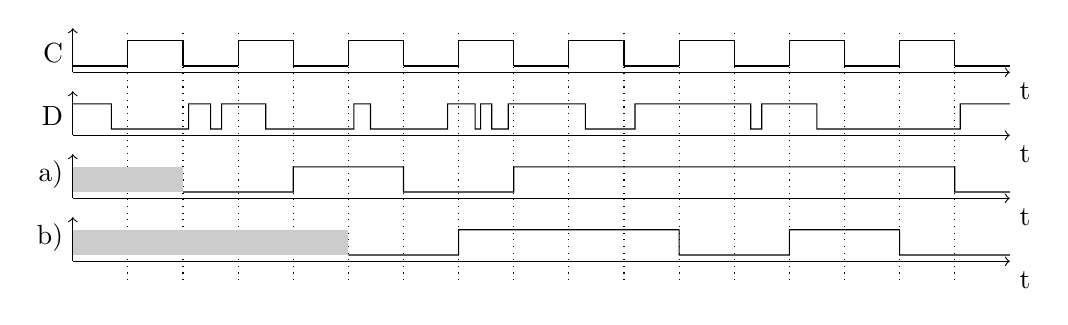
\begin{tikzpicture}[xscale=.7, yscale=.8]

    % helpers
    \def\hAzero{1.4}  \def\hAone{1.8}
    \def\hBzero{0.4}  \def\hBone{0.8}
    \def\hCyzero{3.4} \def\hCyone{3.8}
    \def\hDzero{2.4}  \def\hDone{2.8}

    \def\diff{.4}

    % undefs
    \def\drawundef#1#2{\fill[gray!40] (0, #1) rectangle ++(#2, -\diff);}

    % grid
    \foreach \name/\y in {C/4,D/3,a)/2,b)/1}{
      \draw[<-] (0,\y) -- ++(0,-.7) node[anchor=south east] {\name};
    }
    \foreach \y in {.3,1.3,2.3,3.3}{
      \draw[->] (0,\y) -- ++(17,0) node[anchor=north west] {t};
    }
    \foreach \x in {1,...,16}{
      \draw[dotted] (\x, 0) -- ++(0,4);
    }

    % draw helpers
    \def\drawAt#1#2{\draw (#1,#2) -- ++(1,0);}
    \def\connect#1#2{\draw (#2,#1) -- ++(0,\diff);}

    % draw cycle
    \foreach \x in {0,2,...,16}{
      \drawAt{\x}{\hCyzero}
      \connect{\hCyzero}{\x}
    }
    \foreach \x in {1,3,...,16}{
      \drawAt{\x}{\hCyone}
      \connect{\hCyzero}{\x}
    }

    % draw D
    \def\up{, \hDzero) -- ++(0, \diff) -- (}
    \def\dn{, \hDone)  -- ++(0, -\diff) -- (}
    \draw (0, \hDone) -- (.7 \dn 2.1 \up 2.5 \dn 2.7 \up 3.5 \dn 5.1 \up 5.4 \dn 
                         6.8 \up 7.3 \dn 7.4 \up 7.6 \dn 7.9 \up 9.3 \dn 10.2 \up
                         12.3 \dn 12.5 \up 13.5 \dn 16.1 \up 17, \hDone);

    % draw A
    \def\up{, \hAzero) |- ++(0, \diff) -- (}
    \def\dn{, \hAone)  -- ++(0, -\diff) -- (}
    \drawundef{\hAone}{2}
    \draw (2, \hAzero) -- (4 \up 6 \dn 8 \up 16 \dn 17, \hAzero);

    % draw B
    \def\up{, \hBzero) -- ++(0, \diff) -- (}
    \def\dn{, \hBone)  -- ++(0, -\diff) -- (}
    \drawundef{\hBone}{5}
    \draw (5, \hBzero) -- (7 \up 11 \dn 13 \up 15 \dn 17, \hBzero);

  \end{tikzpicture}
\end{center}

\ex{JK-Flipflops}{6 + 6 + 6 = 18}
\begin{center}
  \noindent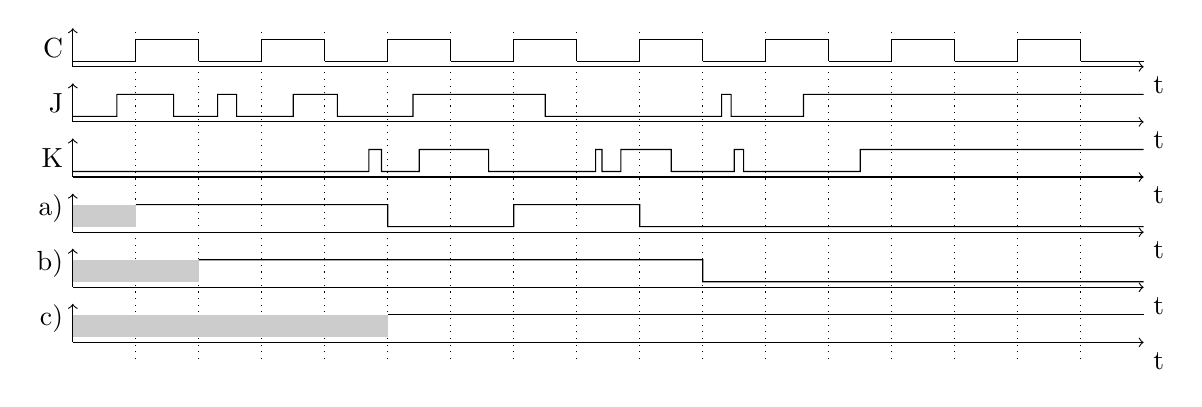
\begin{tikzpicture}[xscale=.8,yscale=.7]

    % helpers
    \def\hAzero{2.4}  \def\hAone{2.8}
    \def\hBzero{1.4}  \def\hBone{1.8}
    \def\hCzero{0.4}  \def\hCone{0.8}
    \def\hCyzero{5.4} \def\hCyone{5.8}
    \def\hJzero{4.4}  \def\hJone{4.8}
    \def\hKzero{3.4}  \def\hKone{3.8}

    \def\diff{.4}

    % undefs
    \def\drawundef#1#2{\fill[gray!40] (0, #1) rectangle ++(#2, -\diff);}
    

    % grid
    \foreach \name/\y in {C/6,J/5,K/4,a)/3,b)/2,c)/1}{
      \draw[<-] (0,\y) -- ++(0,-.7) node[anchor=south east] {\name};
    }
    \foreach \y in {.3,1.3,2.3,3.3,4.3,5.3}{
      \draw[->] (0,\y) -- ++(17,0) node[anchor=north west] {t};
    }
    \foreach \x in {1,...,16}{
      \draw[dotted] (\x, 0) -- ++(0,6);
    }

    % draw cycle
    \def\drawAt#1#2{\draw (#1,#2) -- ++(1,0);}
    \def\connect#1#2{\draw (#2,#1) -- ++(0,\diff);}
    \foreach \x in {0,2,...,16}{
      \drawAt{\x}{\hCyzero}
      \connect{\hCyzero}{\x}
    }
    \foreach \x in {1,3,...,16}{
      \drawAt{\x}{\hCyone}
      \connect{\hCyzero}{\x}
    }

    % draw J
    \def\up{, \hJzero) -- ++(0, \diff) -- (}
    \def\dn{, \hJone)  -- ++(0, -\diff) -- (}
    \draw (0, \hJzero) -- (.7 \up 1.6 \dn 2.3 \up 2.6 \dn 3.5 \up 4.2 \dn 
                          5.4 \up 7.5 \dn 10.3 \up 10.45 \dn 11.6 \up 
                          17, \hJone);
    
    % draw K
    \def\up{, \hKzero) -- ++(0, \diff) -- (}
    \def\dn{, \hKone)  -- ++(0, -\diff) -- (}
    \draw (0, \hKzero) -- (4.7 \up 4.9 \dn 5.5 \up 6.6 \dn 8.3 \up 8.4 \dn 
                           8.7 \up 9.5 \dn 10.5 \up 10.65 \dn 12.5 \up 
                           17, \hKone);

    % draw A
    \def\up{, \hAzero) |- ++(0, \diff) -- (}
    \def\dn{, \hAone)  -- ++(0, -\diff) -- (}
    \drawundef{\hAone}{1}
    \draw (1, \hAone) -- (5 \dn 7 \up 9 \dn 17, \hAzero);

    % draw B
    \def\up{, \hBzero) -- ++(0, \diff) -- (}
    \def\dn{, \hBone)  -- ++(0, -\diff) -- (}
    \drawundef{\hBone}{2}
    \draw (2, \hBone) -- (10 \dn 17, \hBzero);
    
    % draw C
    \def\up{, \hCzero) |- ++(0, \diff) -- (}
    \def\dn{, \hCone)  -- ++(0, -\diff) -- (}
    \drawundef{\hCone}{5}
    \draw (5, \hCone) -- (17, \hCone);
    
  \end{tikzpicture}
\end{center}

\ex{Multifunktions-Schieberegister}{10 + 5 +2 = 17}

\subex{}
\tikzstyle{muxer}=[minimum size=1cm,shape=trapezium,draw,shape border rotate=270]
\tikzstyle{flipflop}=[minimum height=1.5cm,minimum width=1cm,draw]
\usetikzlibrary{shapes}
\newcommand{\flipflop}[2]{
   \node[flipflop,#2] (#1) {};
   \node[right,font=\tiny] (#1-D) at ($(#1.north west) + (0,-10pt)$) {1D};
   \node[left,font=\tiny] (#1-out) at ($(#1.north east) + (0,-10pt)$) {Q};
   \node[isosceles triangle,anchor=west,draw,inner sep=0,minimum width=4pt]
   (#1-clk) at (#1.190) {};
   \node[font=\tiny] (C1) at ($(#1.190) + (1em,0)$) {C1};
   \draw[dashed] (C1) ++(5pt,0) -- (#1.350);
   \path[name path=#1-clk-path] (#1-clk) -- ++(-1em,0) -- ++(0,-5cm);
}
\newcommand{\muxer}[2]{
   \node[muxer,#2] (#1) {};
   \draw 
      let \p1 = ($(#1.bottom left corner) - (#1.bottom right corner)$),
          \n1 = {0.2*veclen(\x1,\y1)}
      in (#1.bottom left corner) +(0,-\n1)   node[anchor=west] (#1-0) {} node[right,font=\tiny] {10}
         (#1.bottom left corner) +(0,-2*\n1) node[anchor=west] (#1-1) {} node[right,font=\tiny] {00}
         (#1.bottom left corner) +(0,-3*\n1) node[anchor=west] (#1-2) {} node[right,font=\tiny] {01}
         (#1.bottom left corner) +(0,-4*\n1) node[anchor=west] (#1-3) {} node[right,font=\tiny] {11};
         \node[anchor=south] (#1-s0) at (#1.-80) {};
         \node[anchor=south] (#1-s1) at (#1.-100) {};
         \path[name path=#1-s0-path] (#1-s0) -- ++(0,-5cm);
         \path[name path=#1-s1-path] (#1-s1) -- ++(0,-5cm);

         \node[font=\tiny,left=3pt of #1-3] (tmp) {0};
         \draw (tmp) ++(3pt,0) -- (#1-3);

         \node[anchor=east] (#1-out) at (#1.top side) {};
}
\newcommand{\drawcommands}[1]{
   \draw[name intersections={of={#1-s0-path and s0}}] (#1-s0) --
   (intersection-1) coordinate (c);
   \fill (c) circle(1pt);
   \draw[name intersections={of={#1-s1-path and s1}}] (#1-s1) --
   (intersection-1) coordinate (c);
   \fill (c) circle (1pt);

}
\newcommand{\drawclock}[1]{
   \draw[name intersections={of={#1-clk-path and clk}}] (#1-clk) -|
   (intersection-1);
   \fill[name intersections={of={#1-clk-path and clk}}] (intersection-1) circle (1pt);
}
\newcommand{\connectbackwards}[3]{
   \draw (#1-out) -- ++(1em,0) coordinate (c1);
   \draw (c1) -- ++(0,#3+1cm) |- ($(#2-0) + (-1em,#3+1cm)$) |- (#2-0);
   \fill (c1) circle (1pt);
}
\noindent\begin{tikzpicture}[node distance=.5cm]
   \path[name path=s0] (0,2em) -- (\linewidth,2em);
   \draw (0,2em) node (s2) {$s_0$} ++(1em,0) -- ++(7cm,0) coordinate (c);
   \draw[dotted] (c) -- ++(1cm,0) coordinate (c2);
   \draw (c2) -- ++(6cm,0);

   \path[name path=s1] (0,1em) -- (\linewidth,1em);
   \draw (0,1em) node (s1) {$s_1$} ++(1em,0) -- ++(7cm,0)
   coordinate (c);
   \draw[dotted] (c) -- ++(1cm,0) coordinate (c2);
   \draw (c2) -- ++(6cm,0);

   \path[name path=clk] (0,0) -- (\linewidth,0);
   \draw (0,0) node (clk) {CLK} ++(1em,0) -- ++(7cm,0)
   coordinate (c);
   \draw[dotted] (c) -- ++(1cm,0) coordinate (c2);
   \draw (c2) -- ++(6cm,0);

   % ASSEMBLY 1 %%%%%%%%%%%%%
   \muxer{mux-7}{above right=1cm and 1cm of s2}
   \flipflop{fl-7}{right=of mux-7}
   \drawcommands{mux-7}
   \drawclock{fl-7}
   %%%%%%%%%%%%%%%%%%%%%%%%%%

   % ASSEMBLY 2 %%%%%%%%%%%%%
   \muxer{mux-6}{right=1cm of fl-7}
   \flipflop{fl-6}{right=of mux-6}
   \drawcommands{mux-6}
   \drawclock{fl-6}
   %%%%%%%%%%%%%%%%%%%%%%%%%%

   \connectbackwards{fl-6}{mux-7}{-10pt}

   \draw (fl-7-out) -- ++(1em,0) coordinate (c3) |- (mux-6-2);
   \fill (c3) circle (1pt);

   \draw (mux-7-out) -- ++(1em,0) |- (fl-7-D);

   \draw (mux-6-out) -- ++(1em,0) |- (fl-6-D);

   \draw[dotted] (fl-6-out) -- ++(1cm,0);

   % ASSEMBLY 3 %%%%%%%%%%%%%
   \muxer{mux-1}{right=2cm of fl-6};
   \flipflop{fl-1}{right=of mux-1};
   \drawcommands{mux-1}
   \drawclock{fl-1}
   %%%%%%%%%%%%%%%%%%%%%%%%%%

   \draw (mux-1-out) -- ++(1em,0) |- (fl-1-D);

   % ASSEMBLY 4 %%%%%%%%%%%%%
   \muxer{mux-0}{right=1cm of fl-1};
   \flipflop{fl-0}{right=of mux-0};
   \drawcommands{mux-0}
   \drawclock{fl-0}
   %%%%%%%%%%%%%%%%%%%%%%%%%%

   \draw (mux-0-out) -- ++(1em,0) |- (fl-0-D);

   \draw (fl-1-out) -- ++(1em,0) |- (mux-0-2);

   \connectbackwards{fl-0}{mux-1}{-10pt}

   \draw (fl-0-out) -- ++(1cm,0);

   \draw (fl-0-out) -- ++(2em,0) coordinate (c1);
   \draw (c1) -- ++(0,1cm) |- ($(mux-7-0) + (-2em,1cm)$) |- (mux-7-2);
   \fill (c1) circle (1pt);

   \draw (c3) -- ++(0,2cm) -| ($(mux-0-0) + (-2em,1cm)$) |- (mux-0-0);

   \foreach \x in {7,6,1,0}{
      \node[above=3cm of fl-\x] (tmp) {D$_\x$};
      \draw[->] (tmp) -- ++(0,-1cm);
      % actual data inputs D_i
      \node[font=\tiny,left=3pt of mux-\x-1] (tmp) {D$_\x$};
      \draw (tmp) ++(5pt,0) -- (mux-\x-1);
   }

   \draw (mux-6-0) -- ++(-1em,0) -- ++(0,0.8cm) -- ++(3cm,0) coordinate (c);
   \draw[dotted] (c) -- ++(1cm,0);

   \draw (mux-1-2) -- ++(-1em,0) coordinate (c);
   \draw[dotted] (c) -- ++(-1em,0);
\end{tikzpicture}

Die Eingänge D$_i$ müssen geeignet beschaltet werden, um die Flipflops zu laden.
Der Übersichtlichkeit halber sind hier keine weiteren Leitungen eingezeichnet.

\subex{}

Für aktuellen Zustand $Q^n$ und gewünschten Folgezustand $Q^{n+1}$ sind folgende
D- bzw. T-Signale nötig.
\begin{center}
\begin{tabular}{>{$}l<{$}|>{$}l<{$}|>{$}c<{$}|>{$}c<{$}}
   Q^n & Q^{n+1} & T & D \\\hline\hline
   0 & 0 & 0 & 0\\
   0 & 1 & 1 & 1\\
   1 & 0 & 1 & 0\\
   1 & 1 & 0 & 1
\end{tabular}
\end{center}

Somit gilt für $T$: 
\begin{equation*}
   T = \comp D Q + D \comp Q = D \oplus Q
\end{equation*}

Das für ein T-Flipflop erforderliche T-Signal kann also wie folgt generiert
werden:

\begin{center}
   \begin{tikzpicture}
      \node[or port,font={=1}] (xor-1) {};
      \node[flipflop,right=of xor-1] (fl-1) {};
      \node[right,font=\tiny] (fl-1-T) at ($(fl-1.north west) + (0,-10pt)$) {T};
      \node[left,font=\tiny] (fl-1-out) at ($(fl-1.north east) + (0,-10pt)$) {Q};
      \node[left,font=\tiny] (fl-1-out-neg) at ($(fl-1.south east) + (0,10pt)$)
      {$\bar{\text{Q}}$};
      \node[isosceles triangle,anchor=west,draw,inner sep=0,minimum width=4pt]
      (fl-1-clk) at ($(fl-1.south west) + (0,10pt)$)  {};

      \node[left=of xor-1.200] (D) {D};
      \draw (D.east) -- (xor-1.200);
      \draw (fl-1-out) -- ++(1em,0) coordinate (c) -- ++(1em,0);
      \draw (fl-1-out-neg) -- ++(1em,0) -- ++(1em,0);
      \fill (c) circle (1pt);
      \draw (c) |- ($(xor-1.160) + (-1em,1cm)$) |- (xor-1.160);
      \draw (xor-1.east) -- ++(1em,0) |- (fl-1-T);
   \end{tikzpicture}
\end{center}

Man ersetzt also alle D-Flipflops durch obige Konstruktion und muss an den
Multiplexern nichts ändern.

\subex{}

Zur Erhöhung der Breite genügt es, die gewünschte Anzahl von
Muxer-Flipflop-Bausteinen hintereinanderzuschalten. Wichtig ist bloß, dass der
erste mit dem letzten und umgekehrt verbunden ist, so wie oben zu sehen.
\end{document}
